\subsection{The executer object} \label{subsec_IExecutionInteractorObject}

A vital implementation that facilitates a high degree of cohesion, whilst maintaining
low coupling and adhering to the \gls{srp} principle is the use of the
\citecode{koks_iexecutioninteractor_2023} interface. The generation process is designed to
execute \enquote{tasks} in a predefined order. By using the
\code{koks_iexecutioninteractor_2023} it is possible to design each of the tasks as
separate classes, entirely complying, or enabling all of the \gls{solid} principles. The 

\begin{figure}[H]
    \centering
    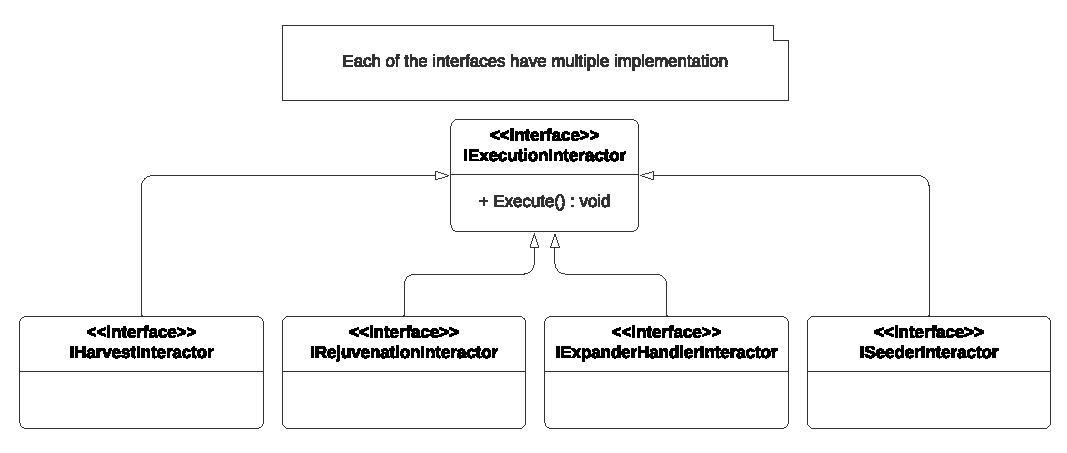
\includegraphics[width=1\textwidth]{figures/class_diagram_iexecutioninteractor.pdf}
    \caption[Plugin Archticture]{Both high cohesion and low coupling by using the \code{koks_iexecutioninteractor_2023}}
    \label{fig_iexecutioninteractor}
  \end{figure}


As depicted in listing \ref{list_CodeGeneratorInteractor}, this design leads to a cohesive
design where all tasks are gracefully executed from a single point in the application.
\lstinputlisting[
  caption={The \citetitle{koks_codegeneratorinteractor_2023}},
  label={list_CodeGeneratorInteractor} ] 
  {Snippets/CodeGeneratorInteractor.cs}